\documentclass[tikz]{standalone}

\usepackage{amsmath}
\usepackage{mathrsfs}
\usetikzlibrary{positioning}

\usepackage{amsmath}
\usepackage{mathrsfs}

\newcommand{\cat}[1]{\mathscr{#1}}
\newcommand{\obj}[1]{\lowercase{#1}}
\newcommand{\objs}[1]{#1}
\newcommand{\mrp}[3]{{#1}:{#2}\to{#3}}
\newcommand{\mrps}[3]{#1(#2,#3)}
\newcommand{\id}[1]{\mathrm{id}_{#1}}
\newcommand{\op}[1]{{#1}^{\mathrm{op}}}
\newcommand{\set}{\mathbf{Set}}
\newcommand{\Top}{\mathsf{Top}}
\newcommand{\blat}{\mathsf{BLat}}
\newcommand{\stone}{\mathsf{Stone}}
\DeclareMathOperator{\dom}{dom}
\DeclareMathOperator{\cod}{cod}
\DeclareMathOperator{\colim}{Colim}
\DeclareMathOperator{\lan}{Lan}
\DeclareMathOperator{\ran}{Ran}
\DeclareMathOperator{\cone}{Cone}
\DeclareMathOperator{\cocone}{Cocone}


\begin{document}
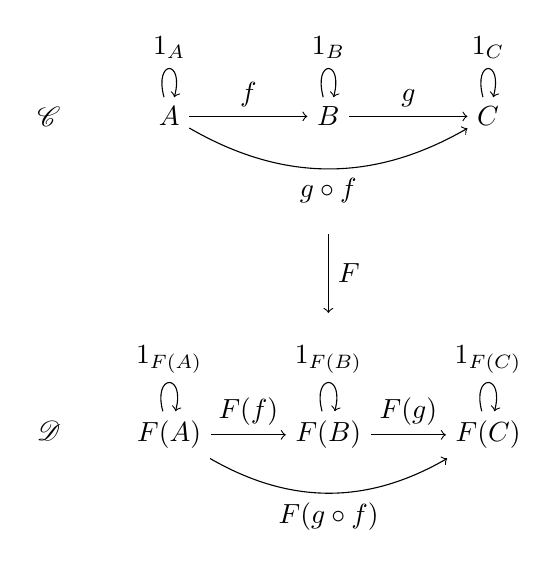
\begin{tikzpicture}
	\node (catc) {$\cat{C}$};
	\node [right=1.0cm of catc] (A) {$A$};
	\node [right=1.5cm of A] (B) {$B$};
	\node [right=1.5cm of B] (C) {$C$};
	\node [below=3.5cm of catc] (catd) {$\cat{D}$};
	\node [below=3.5cm of A] (FA) {$F(A)$};
	\node [below=3.5cm of B] (FB) {$F(B)$};
	\node [below=3.5cm of C] (FC) {$F(C)$};
	\draw [->] (A) to node [above] {$f$} (B);
	\draw [->] (B) to node [above] {$g$} (C);
	\draw [->, bend right] (A) to node [below] {$g\circ f$} (C);
	\draw [->, loop above] (A) to node [above] {$1_A$} (A);
	\draw [->, loop above] (B) to node [above] {$1_B$} (B);
	\draw [->, loop above] (C) to node [above] {$1_C$} (C);
	\draw [->] (FA) to node [above] {$F(f)$} (FB);
	\draw [->] (FB) to node [above] {$F(g)$} (FC);
	\draw [->, bend right] (FA) to node [below] {$F(g\circ f)$} (FC);
	\draw [->, loop above] (FA) to node [above] {$1_{F(A)}$} (FA);
	\draw [->, loop above] (FB) to node [above] {$1_{F(B)}$} (FB);
	\draw [->, loop above] (FC) to node [above] {$1_{F(C)}$} (FC);
	\node [below=1cm of B] (from) {};
	\node [above=1cm of FB] (to) {};
	\draw [->] (from) to node [right] {$F$} (to);
\end{tikzpicture}
\end{document}

